\documentclass{article}
\usepackage{amsmath, amssymb, amsfonts}
\usepackage{tikz} % TikZ is okay with pdflatex
\usepackage{hyperref}
\usepackage{geometry}
\geometry{margin=1in}

\title{\textbf{Complex Equations Showcase \\ for TeXSync Website}}
\author{Developed with \LaTeX\ by TeXSync}
\date{\today}

\begin{document}

\maketitle

\tableofcontents
\newpage

\section{Introduction}

Welcome to \textbf{TeXSync}, the online \LaTeX\ editor.  
Here we showcase the capability to render highly complex mathematical structures.

\section{Calculus}

\subsection{Complex Differentiation}

Let \( f(z) = u(x, y) + i v(x, y) \), then the complex derivative is:
\[
f'(z) = \lim_{\Delta z \to 0} \frac{f(z + \Delta z) - f(z)}{\Delta z}
\]

The Cauchy-Riemann equations are:
\[
\frac{\partial u}{\partial x} = \frac{\partial v}{\partial y}, \quad \frac{\partial u}{\partial y} = -\frac{\partial v}{\partial x}
\]

\subsection{Multivariable Integration}

The volume under a surface \( z = f(x,y) \) is:

\[
V = \iint_D f(x,y) \, dx\, dy
\]

Where \( D \) is the domain of integration.

\subsection{Line Integrals}

For a vector field \( \vec{F} \), the line integral along curve \( C \) is:

\[
\oint_C \vec{F} \cdot d\vec{r} = \oint_C \left( F_x \, dx + F_y \, dy + F_z \, dz \right)
\]

\section{Series and Summations}

The infinite geometric series:

\[
\sum_{n=0}^{\infty} ar^n = \frac{a}{1-r}, \quad \text{for} \quad |r| < 1
\]

The Taylor series expansion for \( e^x \) is:

\[
e^x = \sum_{n=0}^{\infty} \frac{x^n}{n!}
\]

\section{Linear Algebra and Matrices}

A system of linear equations:

\[
\begin{aligned}
2x + 3y - z &= 7 \\
4x - y + 5z &= 3 \\
-6x + 2y + 3z &= 8
\end{aligned}
\]

In matrix form:

\[
\begin{bmatrix}
2 & 3 & -1 \\
4 & -1 & 5 \\
-6 & 2 & 3
\end{bmatrix}
\begin{bmatrix}
x \\ y \\ z
\end{bmatrix}
=
\begin{bmatrix}
7 \\ 3 \\ 8
\end{bmatrix}
\]

\section{Tensor Calculus (Advanced)}

The Riemann curvature tensor:

\[
R^\rho_{\sigma\mu\nu} = \partial_\mu \Gamma^\rho_{\nu\sigma} - \partial_\nu \Gamma^\rho_{\mu\sigma} + \Gamma^\rho_{\mu\lambda} \Gamma^\lambda_{\nu\sigma} - \Gamma^\rho_{\nu\lambda} \Gamma^\lambda_{\mu\sigma}
\]

Einstein field equations:

\[
R_{\mu\nu} - \frac{1}{2} R g_{\mu\nu} + \Lambda g_{\mu\nu} = \frac{8\pi G}{c^4} T_{\mu\nu}
\]

\section{Physics: Quantum Mechanics}

The time-dependent Schrödinger equation:

\[
i\hbar \frac{\partial}{\partial t} \Psi(\mathbf{r}, t) = \left( -\frac{\hbar^2}{2m} \nabla^2 + V(\mathbf{r}, t) \right) \Psi(\mathbf{r}, t)
\]

\section{Graphics: TikZ Example}

\begin{center}
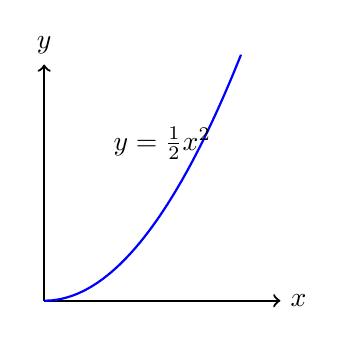
\begin{tikzpicture}
\draw[thick,->] (0,0) -- (3,0) node[right] {$x$};
\draw[thick,->] (0,0) -- (0,3) node[above] {$y$};
\draw[thick,domain=0:2.5,smooth,variable=\x,blue] plot ({\x},{0.5*\x*\x});
\node at (1.5,2) {$y = \frac{1}{2}x^2$};
\end{tikzpicture}
\end{center}

\end{document}